\documentclass[11pt,letterpaper]{article}
\usepackage[lmargin=1in,rmargin=1in,bmargin=1in,tmargin=1in]{geometry}
\usepackage{style/quiz}
\usepackage{style/commands}

% -------------------
% Content
% -------------------
\begin{document}
\thispagestyle{title}


% Quiz 1
\quizsol \textit{True/False}: Any function of one-variable which has a constant rate of change can be written in the form $f(x)= mx + b$ for some values $m$ and $b$. \pspace

\sol The statement is \textit{true}. Suppose the rate of change were 5 and the current value is 2. After one step in time, the value is $2 + 1(5)= 2 + 5= 7$. After another step in time, the value is $7 + 5= 12$, or $2 + 2(5)= 2 + 10= 12$. Generally, after $n$ steps, the value is $2 + n \cdot 5= 5n + 2$, which is a linear function. Generally, if we start with initial value $y_0$ and have a constant rate of change $m$, after $x$ steps, we have $y= y_0 + x \cdot m= mx + y_0$. This is a linear function with $f(x)= y$, $x= x$, $m= m$, and $b= y_0$. But then we see that `any' function which changes at a constant rate is a linear function. We know that a linear function $f(x)= mx + b$ has a constant rate of change---the slope $m$. Therefore, a function is linear if and only if it has a constant rate of change.  \pvspace{1.5cm}



% Quiz 2
\quizsol \textit{True/False}: A break-even point is the point where a revenue and cost function curve intersect. \pspace

\sol The statement is \textit{true}. Suppose that $(x, y)$ is a point in the plane where a revenue curve and a cost curve intersect, i.e. $(x, R(x) )$ and $(x, C(x) )$ are points on the revenue and cost curves, respectively. Then at level of production $x$, the revenue is $y$ and the cost is $y$, i.e. $R(x)= y$ and $C(x)= y$. But then at level of production $x$, we have $y= R(x)= C(x)$. Therefore at $x$, the profit is $P(x):= R(x) - C(x)= y - y= 0$. Therefore, $(x, y)$ is a break-even point. \pvspace{1.5cm}



% Quiz 3
\quizsol \textit{True/False}: If $C(q)$ is a \textit{linear} cost function, then $C(0)$ is the fixed costs and the slope of $C(q)$ is the marginal cost, i.e. the production cost per item. \pspace

\sol The statement is \textit{true}. Suppose that $C(q)$ is the cost of producing $q$ items. The fixed costs are the costs that are incurred regardless of the level of production. Because if $q > 0$ some product is produced, the level of production corresponding to no production is $q= 0$. But then the fixed costs (the costs at a level of production of zero) are $C(0)$. The marginal cost at a level of production $q$ is the additional cost of producing one additional item, i.e. $C(q + 1) - C(q)$. Suppose that $C(q)$ were linear; that is, $C(q)= mq + b$ for some $m, b$, where $m$ is the slope. Notice if we use the points $(q, C(q) )$ and $(q + 1, C(q + 1) )$ to compute the slope of $C(q)$, we obtain\dots
	\[
	m= \dfrac{\Delta C}{\Delta q}= \dfrac{C(q + 1) - C(q)}{(q + 1) - q}= \dfrac{C(q + 1) - C(q)}{1}= C(q + 1) - C(q).
	\]
But then the slope of the linear function $C(q)$ is the marginal cost of production. \pvspace{1.5cm}



% Quiz 4
\quizsol \textit{True/False}: If the CPI (Consumer Price Index) was 253.80 last year and it is 284.75 this year, then the inflation rate from last year to this year was 12.91\%. \pspace

\sol The statement is \textit{false}. The given two CPI's (measured from the same baseline), we can find the quotient of the new CPI and the old CPI and recognize it as a percentage increase (or decrease in the case of deflation). This percentage increase/decrease is the inflation/deflation rate. Therefore, we have $284.75/253.80 \approx 1.1219$, i.e. $284.75= 253.80(1.1219)= 253.80(1 + 0.1219)$. We can see that $1.1219= 1 + 0.1219$ represents a percent increase of 12.19\%---not 12.91\%. Note that some will say that the inflation rate should be calculated from the expression $\frac{\text{new CPI} - \text{old CPI}}{\text{old CPI}}$. Using this, we have $\frac{284.75 - 253.80}{284.75}= \frac{30.95}{253.80} \approx 0.1219 \squiggle 12.19\%$. These give equivalent answers in the case of inflation:
	\[
	\frac{\text{new CPI} - \text{old CPI}}{\text{old CPI}}= \frac{\text{new CPI}}{\text{old CPI}} - \frac{\text{old CPI}}{\text{old CPI}}= \frac{\text{new CPI}}{\text{old CPI}} - 1.
	\]
We already computed $\text{new CPI}/\text{old CPI}$ above---the minus one merely makes it simpler to recognize the percentage increase. However, in the case of deflation, one would need take the absolute value of this difference in the case of deflation---a disadvantage from the original method. [Unless one interprets a negative inflation rate as deflation.] \pvspace{1.5cm}



% Quiz 5
\quizsol \textit{True/False}: If someone invests \$1,500 at 5.4\% annual interest, compounded quarterly, then in 5~years the investment is worth $\$1500 \left( 1 + \dfrac{0.054}{4} \right)^5 \approx \$1604.02$. \pspace

\sol The statement is \textit{false}. If we have a principal of $P$ invested at an annual interest rate $r$, compounded discretely $k$ times per year for $t$ years, then the amount that $P$ has grown to after $t$ years is given by\dots
	\[
	P \left( 1 + \dfrac{r}{k} \right)^{kt}
	\]
We know that the principal is $P= 1500$ and that the annual interest rate is $r= 0.054$ . Because the interest is compounded quarterly (four times per year), we know also that $k= 4$. Finally, because $t= 5$, we have
	\[
	P \left( 1 + \dfrac{r}{k} \right)^{kt}= \$1500 \left( 1 + \dfrac{0.054}{4} \right)^{4 \cdot 5} \approx \$1500 (1.0135)^{20} \approx \$1500(1.30760045) \approx \$1961.40
	\]
The power on the given expression should have been 20---the number of times that the amount has been compounded. \pvspace{1.5cm}



% Quiz 6
\quizsol \textit{True/False}: At the start of each month, Carter deposits \$150 into an account that earns 0.3\% yearly annual interest, compounded monthly. To compute how much Carter will have in 8~years, one would need to calculate the future value for general ordinary annuity. \pspace

\sol The statement is \textit{false}. A general annuity is where the yearly payment and compound rates are not the same, while a simple annuity is where they occur at the same rate. Because the deposits and interest occur monthly, this is a simple annuity. An ordinary annuity is where the payments occur at the end of a period, while an annuity due are where payments occur at the start of the month. Carter deposits the month at the start of the month; therefore, this is an annuity due. Because we want to know how much money is accrued at the end of this time period, we are seeking a future value. Therefore, Carter needs to compute a future value for a simple ordinary annuity. 





\newpage





% Quiz 7
\quizsol \textit{True/False}: Suppose Rasheed takes out an amortized loan for \$57,000 at an annual interest rate of 6.7\%, compounded monthly. He makes monthly payments of \$1,752.19 for 3 years. The total interest he pays on this loan is $\$1752.19(36) - \$57000 = \$6078.84$. \pspace

\sol The statement is \textit{true}. If he pays \$1,752.19 per month for 3~years, he makes a total of $3 \cdot 12= 36$~payments. Then the total payment is $36 \cdot \$1752.19= \$63,078.84$. Because this repays both the loan and the interest, we know that the difference between the total amount paid and the loan value must be the interest. But then we have $\$63,078.84 - \$57,000= \$6,078.84$ in interest. \pvspace{1.5cm}




% Quiz 8
\quizsol \textit{True/False}: Given a dataset $\{ (x_i, y_i) \}$, a simple linear regression line $\widehat{y}= b_0 + b_1x$, is the line which minimizes the sum of the squares of the errors for this model. \pspace

\sol The statement is \textit{true}. Given a linear model $\widehat{y}= b_0 + b_1 x$, for each $x_i$ in the dataset, we can compute a predicted $y$-value---namely $\widehat{y}_i:= b_0 + b_1 x_i$. There is then an associated error/residual to this prediction: $e_i= y_i - \widehat{y}_i$. There is then a total square error for this model: $\displaystyle \sum_i e_i^2= \sum (y_i - \widehat{y}_i)^2$. A simple linear regression is a linear model which minimizes this sum for the given dataset. \pvspace{1.5cm}


% Quiz 9
\quizsol \textit{True/False}: Suppose you have a dataset $\{ (x_i, y_i ) \}$, where $x$ is the number of hours spent at the mall $y$ is the amount of money left in someone's wallet. If a linear regression model performed on this dataset and results in $\widehat{y}= 27.1 - 4.5x$. Then the model predicts that $x$ and $y$ are negatively correlated and that, on average, you spend \$4.50 every hour at the mall. \pspace

\sol The statement is \textit{true}. We have a linear model $\widehat{y}= 27.1 - 4.5x$ so that $b_0= 27.1$, i.e. $y$-intercept $27.1$, and $b_1= -4.5$, i.e. slope $-4.5$. Because $b_1 < 0$, the model predicts that $x$ and $y$ are negatively correlated. Interpreting the slope $-4.5= \frac{-4.5}{1}= \frac{\Delta y}{\Delta x}$, we see that for every increase of 1 in $x$, there is a decrease of 4.5 in $y$, i.e. for every additional hour spent at the mall, you lose (spend) \$4.50. \pvspace{1.5cm}



% Quiz 10
\quizsol \textit{True/False}: Let $A$ and $B$ be events. Then $P(A \text{ and } B)= P(A) \cdot P(B)$. \pspace

\sol The statement is \textit{false}. This is generally true only when $A$ and $B$ are independent events. Generally, we have $P(A \text{ and } B)= P(A) \cdot P(B \;|\; A)$ or equivalently $P(A \text{ and } B)= P(B) P(A \;|\; B)$. That is, we find the probability of $B$ occurring and then $A$ occurring given that $B$ occurs, or the probability that $A$ occurs given that $B$ occurs. If $A$ and $B$ are independent, then their occurrence/non-occurrence does not affect the occurrence/non-occurrence of the other, i.e. it does not affect their probability of occurrence. In this case, $P(A \;|\; B)= P(A)$ and $P(B \;|\; A)= B$. But then $P(A \text{ and } B)= P(A) P(B)$. However, if $A$ and $B$ are \textit{not} independent, these probabilities can be different. For instance, imagine taking an exam. Let $A$ be the event that you score at least an 85 and $B$ be the event where you pass an exam. Then $P(A \;|\; B)$ is the probability that you score at least an 85 given that you pass the exam. Who knows what this is? However, we know that $P(B \;| A)$, i.e. the probability that you pass the exam given that you score at least an 85\%, is certainly 1---if you received at least an 85\%, you passed! Observe that these probabilities are not the same. Moreover, knowing that you passed the exam certainly increases the likelihood that you received 85\% or higher. If one wanted $P(A \text{ and } B)$, one cannot then simply multiply $P(A)$ and $P(B)$. \pvspace{1.5cm}



% Quiz 11
\quizsol \textit{True/False}: If $A$ and $B$ are events, then $P(A \text{ or } B)= P(A) + P(B) - P(A \text{ and } B)$. \pspace

\sol The statement is \textit{true}. We can always add the probabilities of events $A$ and $B$ to find $P(A \text{ or } B)$; however, we then may overcount events which occurred in both $A$ and $B$. What would this overcount be? The probability of the events that are in both $A$ and $B$ is precisely $P(A \text{ and } B)$. Therefore, we have $P(A \text{ or } B)= P(A) + P(B) - P(A \text{ and } B)$. If $A$ and $B$ are disjoint, i.e. share no events in common, we know that $P(A \text{ and } B)= 0$, because $A$ and $B$ cannot occur at the same time. But then if $A$ and $B$ are disjoint events, we have $P(A \text{ or } B)= P(A) + P(B)$. \pvspace{1.5cm}



% Quiz 12
\quizsol \textit{True/False}: Suppose you play a game of chance, and call the amount you win or lose per game $X$ and label by $EX$ the expected value of $X$. Then if $EX= \$4.30$, the expected value of $X$, then if you played the game `enough times' and averaged the net total amount you won/lost, you could expect to win approximately \$4.30 per game on average. \pspace

\sol The statement is \textit{true}. We know that the expected value of a discrete random variable $X$ is\dots
	\[
	EX= \sum x P(X= x)
	\]
That is, the expected value is the sum of the values times their probability. [One could then say, it is the sum of the values weighted by their probability.] To see why this measures the amount you win/lose on average, suppose you have a game where you either win \$10 or lose \$5. If you wanted to find the average amount you have won/lost after playing the game $n$ times, you have\dots
	\[
	\begin{aligned}
	\text{Average Amount}&= \dfrac{\$10 \cdot \text{Times Won} + (-\$5) \cdot \text{Times Lost}}{n} \\
	&= \dfrac{\$10 \cdot \text{Times Won}}{n} + \dfrac{-\$5 \cdot \text{Times Lost}}{n} \\
	&= \$10 \cdot \dfrac{\text{Times Won}}{n} + (-\$5) \cdot \dfrac{\text{Times Lost}}{n} \\
	&\approx \$10 \cdot \text{Probability Won} + (-\$5) \cdot \text{Probability Lost}
	\end{aligned}
	\] 
The last approximation becomes more and more accurate the more games you play because $\frac{\text{times won}}{n}$ and $\frac{\text{times lost}}{n}$ approach the probability of winning or losing, respectively, as $n$ gets larger. Therefore, if $EX= \$4.30 > 0$, we expect that if we played this game a `large' number of times, the average amount we won per game was \$4.30. 





\newpage





% Quiz 13
\quizsol \textit{True/False}: The normal distribution given by $N(-5.6, 2.2)$ has mean $\mu= -5.6$ and standard deviation $\sigma= 2.2$. \pspace

\sol The statement is \textit{true}. The notation $N(\mu, \sigma)$ denotes a normal distribution with mean $\mu$ and standard deviation $\sigma$. Therefore, $N(-5.6, 2.2)$ denotes a normal distribution with mean $\mu= -5.6$ and standard deviation $\sigma= 2.2$. \pvspace{1.5cm}



% Quiz 14
\quizsol \textit{True/False}: Suppose Alice and Bob took an exam with scores that were normally distributed. Alice received a score that had a $z$-score of $-3.15$. Bob received a score that had a $z$-score of $1.18$. Because Alice's score had a $z$-score that was larger in absolute value, her score was more `unusual' and she did better on the exam. \pspace

\sol The statement is \textit{false}. We know the larger $|z|$, the more `unusual' the score. This is because the $z$-score measures the number of standard deviations away from the mean a value is. For a normal distribution, the more negative or positive that $z$ is, the further the value must be from the mean. Because $|-3.15|= 3.15 > 1.18= |1.18|$, we know that Alice's score is more `unusual' than Bob's. However, if $z < 0$, the value is below the mean; if $z= 0$, the value is equal to the mean; if $z > 0$, the value is above the mean. Because $z= -3.15 < 0$, Alice received a below average exam score. And because $1.18 > 0$, Bob received an above average exam score. Therefore, Alice did worse than Bob. \pvspace{1.5cm}



% Quiz 15
\quizsol \textit{True/False}: If you take simple random samples of size 15 from a distribution with mean 130 and standard deviation 25, the resulting distribution of sample means is $N(130, 25/\sqrt{15}) \approx N(130, 6.45497)$. \pspace

\sol The statement is \textit{false}. If a random variable $X$ has a distribution with mean $\mu$ and (finite) standard deviation $\sigma$, the Central Limit Theorem (CLT) says that the distribution of sample means, $\overline{X}$, of size $n$ has distribution $N(\mu, \sigma/\sqrt{n})$ so long as at least one of the following criterion are met: the underlying distribution is normal, i.e. you are sampling from $N(\mu, \sigma)$, or the sample size is `sufficiently large' (e.g., $n \geq 30$). We were not told that the underlying distribution was normal. Because the sample size is $15 < 30$, the sample size is not sufficiently large enough to meet the criterion of the Central Limit Theorem. Therefore, it is not necessarily the case that the distribution of $\overline{X}$ is $N(130, 25/\sqrt{15}) \approx N(130, 6.45497)$. \pvspace{1.5cm}



% Quiz 16
\quizsol \textit{True/False}: Suppose that a support for a particular bill is approximately 34\%, i.e. 34\% of the population supports the bill. Then among a population of 1,000 randomly chosen individuals, the distribution of the number of people supporting the bill is approximately $N(340, 14.98)$. \pspace

\sol The statement is \textit{true}. An individual either supports the bill or not. We are selecting a fixed number of individuals---namely 1,000---with fixed probability of support---namely 34\%. We assume that the individuals opinions on the bill are independent from each other. [We assume also that the population is `large' relative to this sample.] The support for the bill then has binomial distribution $B(1000, 0.34)$. This would be cumbersome to work with. We know that $np= 1000(0.34)= 340 \geq 10$ and $n(1 - p)= 1000(1 - 0.34)= 1000(0.66)= 660 \geq 10$. Therefore, we can use the normal approximation to the binomial distribution. For counts, the normal approximation to the binomial distribution is $N(np, \sqrt{np(1 - p)})= N(1000 \cdot 0.34, \sqrt{1000 \cdot 0.34 \cdot 0.66}) \approx N(340, 14.98)$. \pvspace{1.5cm}



% Quiz 17
\quizsol \textit{True/False}: If $X$ is a sample count from a population of size 1,000 with $p= 0.50$, then $X$ is approximately distributed as $N(500, 15.81)$. \pspace

\sol The statement is \text{true}. Because $np= 1000(0.50)= 500 \geq 10$ and $n(1 - p)= 1000(1 - 0.50)= 1000 (0.50)= 500 \geq 10$, we know that the Central Limit Theorem applies. Therefore, we can approximate the binomial distribution of $X$, i.e. $B(1000,0.50)$, with the normal distribution $N(np, \sqrt{np(1 - p)})$. But then we have $N(1000 \cdot 0.50, \sqrt{1000 \cdot 0.50 (1 - 0.50)})= N(500, 15.81)$. \pvspace{1.5cm}



% Quiz 18
\quizsol \textit{True/False}: If $\mathbf{u}= \begin{pmatrix} 1 & 2 & 3 \end{pmatrix}$ and $\mathbf{v}= \begin{pmatrix} -2 & 3 & 1 \end{pmatrix}$, then $\mathbf{u} \cdot \mathbf{v}= \begin{pmatrix} -2 & 6 & 3 \end{pmatrix}$. \pspace

\sol The statement is \textit{false}. The dot product of two vectors is \textit{not} simply the vector of the product of the components. Rather, the dot product of two vectors is the \textit{sum} of the product of the components of the vectors. We then have\dots
	\[
	\mathbf{u} \cdot \mathbf{v}= \sum_i u_i v_i= 1(-2) + 2(3) + 3(1)= -2 + 6 + 3= 7 
	\] \pvspace{1.5cm}



% Quiz 19
\quizsol \textit{True/False}: If $A$ is a $10 \times 8$ matrix and $B$ is a $8 \times 12$ matrix, then $AB$ is a $10 \times 12$ matrix. \pspace

\sol The statement is \textit{true}. If $A$ is a $m \times n$ matrix and $B$ is a $r \times s$ matrix, we can form the matrix product $AB$ if and only if $n= r$. If so, the result will be a $m \times s$ matrix. Here, we have $m= 10$, $n= 8$ and $r= 8$, $s= 12$. Because $n= 8= r$, we can form the product $AB$. The result, will be a matrix of size $m \times s= 10 \times 12$. 





\newpage





% Quiz 20
\quizsol \textit{True/False}: Suppose the matrix given below is the RREF form of an augmented matrix coming from a linear system of equations. Then the original system had 3 linear equations in 5 variables and the system has 3 free variables. 
	\[
	\begin{pmatrix}
	1 & 3 & 0 & 0 & 0 & 5 \\
	0 & 0 & 1 & 2 & 1 & -1 \\
	0 & 0 & 0 & 0 & 0 & 0 \\
	\end{pmatrix}
	\] \pspace

\sol The statement is \textit{true}. Because there were 3 rows, we know that there were three linear equations under consideration. The last column corresponds to the `solutions' while the other columns corresponds to variables in the equation. Therefore, there were $6 - 1= 5$ original variables. The free variables correspond to non-pivot columns. We highlight the pivot columns below
	\[
	\begin{pmatrix}
	\boxed{1} & 3 & 0 & 0 & 0 & 5 \\
	0 & 0 & \boxed{1} & 2 & 1 & -1 \\
	0 & 0 & 0 & 0 & 0 & 0 \\
	\end{pmatrix}
	\] 
As there were 2 pivot columns, there must be $5 - 2= 3$~free variables. \pvspace{1.5cm}



% Quiz 21
\quizsol \textit{True/False}: The region shown below is bounded. 
	\[
	\fbox{
	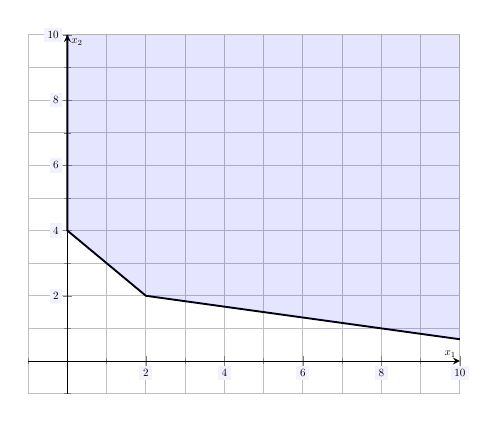
\begin{tikzpicture}[scale=0.8,every node/.style={scale=0.5}]
	\begin{axis}[
	grid=both,
	axis lines=middle,
	ticklabel style={fill=blue!5!white},
	xmin= -1, xmax=10,
	ymin= -1, ymax=10,
	xtick={0,2,4,6,8,10},
	ytick={0,2,4,6,8,10},
	minor tick = {-1,0,1,...,10},
	xlabel=\(x_1\),ylabel=\(x_2\),
	]
	\draw[line width=0.03cm] (10,2/3) -- (2,2) -- (0,4) -- (0,10);
	\draw[line width=0.01cm,fill= blue,opacity=0.1] (10,2/3) -- (2,2) -- (0,4) -- (0,10) -- (10,10) -- (10,2/3);
	\end{axis}
	\end{tikzpicture}
	}
	\] \pspace

\sol The statement is \textit{false}. Because there are points, $(x, y)$ with arbitrarily large coordinates, the region is unbounded. That is, there is no `ball' of fixed size which can enclose the region. Therefore, the region is unbounded. 





\newpage





% Quiz 22
\quizsol \textit{True/False}: \textit{Any} linear function on \textit{any} bounded, nonempty region has a maximum and minimum. \pspace

\sol The statement is \textit{true}. This follows from the Fundamental Theorem of Linear Programming. The Fundamental Theorem of Linear Programming states that any linear function on a nonempty, bounded region has a maximum and minimum value. Furthermore, these maximum and minimum values occur at corner points for the region. \pvspace{1.5cm}



% Quiz 23
\quizsol \textit{True/False}: The initial simplex tableau for a standard maximization problem is found below. This tableau implies that the original system had 3 inequalities and 5 variables. \par
	\begin{table}[!ht]
	\centering
	\begin{tabular}{rrrrrr}
	$1$ & $0$ & $-3$ & $1$ & $0$ & $25$ \\
	$-$1 & $2$ & $3$ & $0$ & $1$ & $20$ \\
	$-1$ & $-1$ & $2$ & $0$ & $0$ & $0$ 
	\end{tabular}
	\end{table} \pspace

\sol The statement is \textit{false}. First, we `split' the table as follows: \par
	\begin{table}[!ht]
	\centering
	\begin{tabular}{rrrrr|r}
	$1$ & $0$ & $-3$ & $1$ & $0$ & $25$ \\
	$-$1 & $2$ & $3$ & $0$ & $1$ & $20$ \\ \hline
	$-1$ & $-1$ & $2$ & $0$ & $0$ & $0$ 
	\end{tabular}
	\end{table} \par
The last row corresponds to the function. All other rows correspond to inequalities in the original system of inequalities. Therefore, there were two inequalities in the original system (excluding the inequalities enforcing non-negativity of our variables). For each such inequality, we introduce a slack variable. Therefore, there are 2 slack variables. Each column, except for the last which corresponds to `solutions', corresponds to a variable. Therefore, there are $6 - 1= 5$ total variables. Because 2 of them are slack variables, there were $5 - 2= 3$ variables in the original system of inequalities. 





\end{document}